\documentclass[aspectratio=169,10pt]{beamer}

% ============================== SETUP ==============================
\usepackage{fontspec}
\setmainfont{Noto Sans}
\setsansfont{Noto Sans}
\newfontfamily\monofont{Noto Sans Mono}

\usetheme[progressbar=frametitle,numbering=counter,background=light]{metropolis}
\setbeamertemplate{navigation symbols}{}
\setbeamertemplate{frame numbering}[counter]

\usepackage{tikz}
\usetikzlibrary{arrows.meta,positioning,calc,shapes.geometric}
\usepackage{tcolorbox}
\tcbuselibrary{skins}
\usepackage{graphicx}
\usepackage{adjustbox}
\usepackage{pgfpages}
\graphicspath{{slides_assets/}}

% ---- toggle: false = presentation only, true = adds speaker-note pages
\newif\ifshownotes
\shownotesfalse
\ifshownotes
  \setbeameroption{show notes on second screen=right}
\fi

% ============================== PALETTE (light) ==============================
\definecolor{bg}{HTML}{F7F9FC}
\definecolor{bgpanel}{HTML}{EFF3F9}
\definecolor{bgpanel2}{HTML}{E7ECF3}
\definecolor{line}{HTML}{8C9AB0}
\definecolor{linesoft}{HTML}{B4C0D1}
\definecolor{ink}{HTML}{16202E}
\definecolor{inkdim}{HTML}{435166}
\definecolor{inkfaint}{HTML}{7C8CA3}
\definecolor{accent}{HTML}{B8710F}
\definecolor{accenttwo}{HTML}{0E7D6F}
\definecolor{warning}{HTML}{C2464E}
\definecolor{accentinkon}{HTML}{FFF6E9}
\definecolor{accenttwoinkon}{HTML}{EAFBF6}

\setbeamercolor{background canvas}{bg=bg}
\setbeamercolor{normal text}{fg=ink,bg=bg}
\setbeamercolor{frametitle}{fg=ink,bg=bg}
\setbeamercolor{framesubtitle}{fg=inkdim}
\setbeamercolor{progress bar}{fg=accent,bg=linesoft}
\setbeamercolor{title separator}{fg=accent}
\setbeamercolor{alerted text}{fg=warning}
\setbeamercolor{example text}{fg=accenttwo}
\setbeamercolor{page number in head/foot}{fg=inkdim}
\setbeamerfont{page number in head/foot}{family=\monofont,size=\small,series=\bfseries}
\setbeamerfont{frametitle}{series=\bfseries,size=\Large}
\setbeamerfont{framesubtitle}{family=\monofont,size=\scriptsize}
\setbeamertemplate{frametitle continuation}{}

\setbeamertemplate{itemize item}{\textcolor{accenttwo}{\scriptsize$\blacktriangleright$}}
\setbeamertemplate{itemize subitem}{\textcolor{inkdim}{\tiny$-$}}
\setlength{\parskip}{4pt}

% ============================== MACROS ==============================
\newcommand{\muD}{\ensuremath{\mu}D3TN}
\newcommand{\eyebrow}[1]{\textcolor{inkdim}{\small\monofont \MakeUppercase{#1}}}

\newtcbox{\chip}[1][]{on line, arc=9pt, colframe=line, colback=bgpanel2,
  boxrule=0.8pt, top=4pt, bottom=4pt, left=10pt, right=10pt,
  fontupper=\monofont\normalsize, before upper={\color{ink}}, #1}
\newtcbox{\chipstrong}[1][]{on line, arc=9pt, colframe=accent, colback=bgpanel2,
  boxrule=1pt, top=4pt, bottom=4pt, left=10pt, right=10pt,
  fontupper=\monofont\normalsize\bfseries, before upper={\color{ink}}, #1}
\newtcbox{\milestone}[1][]{on line, arc=10pt, colframe=accenttwo, colback=accenttwo,
  boxrule=0pt, top=5pt, bottom=5pt, left=14pt, right=14pt,
  fontupper=\monofont\normalsize\bfseries, before upper={\color{accenttwoinkon}}, #1}

% \bigfig maximizes a tikzpicture to fill the space freed by removing
% titles/prose: it scales up to whichever of width/height is tighter.
\newcommand{\bigfig}[2][0.82\textheight]{\begin{center}\adjustbox{max width=\linewidth,max height=#1}{#2}\end{center}}

% \photo frames a real photo consistently with the vector panels: a thin
% rule border, scaled to fit within the given width/height box.
\newcommand{\photo}[3]{\adjustbox{cfbox=line 1.4pt 0pt,max width=#1,max height=#2}{\includegraphics{#3}}}

\newcommand{\led}[1]{\tikz[baseline=-0.6ex]{\filldraw[#1,draw=#1] (0,0) circle (2.1pt);}}

% simple padlock glyph, centered at (x,y), in the given color
\newcommand{\lockicon}[3]{%
  \draw[#3,fill=#3,rounded corners=2pt] (#1-0.32,#2-0.30) rectangle (#1+0.32,#2+0.22);
  \draw[#3,line width=2.4pt] (#1-0.2,#2+0.22) arc (180:0:0.2);
}

\newtcolorbox{cardbox}{colback=bgpanel2, colframe=line, boxrule=0.6pt,
  arc=6pt, left=14pt, right=14pt, top=7pt, bottom=7pt, coltext=ink}

\tikzset{
  panel/.style={draw=line, line width=1pt, fill=bgpanel, rounded corners=3pt},
  panel2/.style={draw=line, line width=1pt, fill=bgpanel2, rounded corners=3pt},
  accentbox/.style={draw=accent, fill=accent, rounded corners=3pt},
  accenttwobox/.style={draw=accenttwo, fill=accenttwo, rounded corners=3pt},
  warnbox/.style={draw=warning, line width=1.1pt, fill=bgpanel2, rounded corners=3pt},
  arrline/.style={-{Latex[length=2.8mm,width=2mm]}, line width=1.3pt, draw=inkdim},
  accline/.style={-{Latex[length=2.4mm,width=1.7mm]}, line width=1.3pt, draw=accenttwo},
  dimline/.style={line width=0.9pt, draw=inkdim, dash pattern=on 3pt off 3pt},
  lbl/.style={font=\monofont\normalsize, text=inkdim},
  lblf/.style={font=\monofont\normalsize, text=inkdim},
  lbli/.style={font=\monofont\normalsize, text=ink},
  lbld/.style={font=\bfseries\sffamily\Large, text=ink},
}

\title{CSPCL}
\author{Mathias Durat}
\date{STINT 2026}
\hypersetup{pdftitle={CSPCL --- STINT 2026},pdfauthor={Mathias Durat, Sarah Theoulle, Hugo Ponthieu, Tristan-Mihai Radulescu, Olivier De Jonck\`ere}}

\begin{document}

% ============================== SLIDE 1 — TITLE ==============================
\begin{frame}[plain]
\vspace{2pt}

\eyebrow{STINT 2026 - Leuven, Belgium}\\[16pt]
{\fontsize{54}{54}\selectfont\bfseries\color{ink} CSPCL}\\[10pt]
{\Large\color{ink} A stepwise, non-disruptive transition to Delay-Tolerant\\ Networking for CubeSat operators.}\\[22pt]

\chip{Mathias Durat} \chip{Sarah Theoulle} \chip{Hugo Ponthieu} \chip{Tristan-Mihai Radulescu} \chip{Olivier De Jonck\`ere}

\vspace{7pt}

\vspace{8pt}
\chip{LIRMM $\cdot$ Polytech Montpellier $\cdot$ CSUM}

\vfill

\begin{tikzpicture}[baseline=0pt]
  \foreach \x/\w in {0.4/2.2,2.9/1.4,4.6/2.8,7.7/0.9,8.9/1.9,11.1/1.1,12.5/2.3}
    \fill[accenttwo] (\x,0) rectangle ++(\w,0.22);
  \fill[accent] (9.9,0) rectangle ++(0.55,0.22);
  \draw[inkdim,line width=0.5pt] (0,-0.14) -- (15.2,-0.14);
\end{tikzpicture}

\note{Good morning. I'm going to talk about CSPCL --- a way to bring Delay-Tolerant Networking to CubeSats that already fly the CubeSat Space Protocol, without touching what already works. This is joint work with Sarah Theoulle, Hugo Ponthieu, Tristan-Mihai Radulescu and Olivier De Jonck\`ere, from LIRMM and Polytech Montpellier, developed around the Centre Spatial de l'Universit\'e de Montpellier's upcoming CubeSat missions.}
\end{frame}

% ============================== SLIDE 2 — MEET CSUM ==============================
\begin{frame}{Meet CSUM}

\vfill
\centering
\begin{columns}[c]
\begin{column}{0.4\textwidth}\centering
\photo{\linewidth}{0.55\textheight}{csum_map.png}
\end{column}
\begin{column}{0.56\textwidth}\centering
\photo{\linewidth}{0.55\textheight}{csum_building.png}
\end{column}
\end{columns}

\vspace{16pt}
\chip{Montpellier, France} 
\vfill

\note{This work exists because of a real customer: CSUM, the Centre Spatial de l'Universit\'e de Montpellier, based here in Montpellier. They're preparing an upcoming 12U CubeSat mission, and like most university-scale CubeSat teams, they operate with a small team and a small budget --- nothing like a national space agency's headcount.}
\end{frame}

% ============================== SLIDE 3 — CONTROL ROOM ==============================
\begin{frame}{The control room}

\vfill
\centering
\photo{0.82\linewidth}{0.66\textheight}{control_room.png}

\vspace{16pt}
\vfill

\note{This is CSUM's control room today. Real operations, run by hand, by a small team, on a stack they know cold. It's not glamorous, but it's production, and it's their accumulated expertise. You don't replace that in a day, and you don't get permission to try. That's the reality any DTN transition has to respect.}
\end{frame}

% ============================== SLIDE 4 — THE PROBLEM ==============================
\begin{frame}{The problem}

\vfill
\centering{\Huge\color{ink}\bfseries How to go DTN,\\ non-intrusively?}
\vfill

\note{So here is the actual question this talk answers: how do you bring Delay-Tolerant Networking to a fleet like CSUM's, without touching the stack that already flies?}
\end{frame}

% ============================== SLIDE 5 — CSP REALITY ==============================
\begin{frame}{CSP over CAN}

\vfill
\bigfig[0.6\textheight]{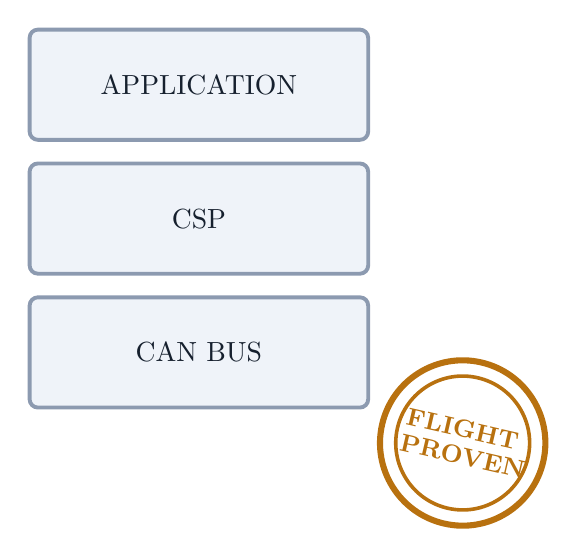
\begin{tikzpicture}
\draw[panel,line width=1.4pt] (0,4.6) rectangle (4.3,6.0); \node[lbli] at (2.15,5.3) {APPLICATION};
\draw[panel,line width=1.4pt] (0,2.9) rectangle (4.3,4.3); \node[lbli] at (2.15,3.6) {CSP};
\draw[panel,line width=1.4pt] (0,1.2) rectangle (4.3,2.6); \node[lbli] at (2.15,1.9) {CAN BUS};
\draw[accent,line width=2.2pt,rotate around={-13:(5.5,0.75)}] (5.5,0.75) circle (1.05);
\draw[accent,line width=1.3pt,rotate around={-13:(5.5,0.75)}] (5.5,0.75) circle (0.85);
\node[font=\monofont\small\bfseries,text=accent,rotate=-13] at (5.5,0.93) {FLIGHT};
\node[font=\monofont\small\bfseries,text=accent,rotate=-13] at (5.5,0.58) {PROVEN};
\end{tikzpicture}}

\vspace{16pt}
\centering{\Large\color{accent}\bfseries "It just works."}
\vfill

\note{CubeSat operators like CSUM already have a working stack. Their onboard software runs the CubeSat Space Protocol, CSP, directly over a CAN bus --- the wired, onboard side of the architecture. This stack is flight-proven, and it just works. But that phrase cuts both ways: a transition toward DTN has a real cost, in engineering time and risk, and a small actor doesn't necessarily get to pay it.}
\end{frame}

% ============================== SLIDE 6 — TWIST, PART 1 ==============================
\begin{frame}{One small issue}

\vfill
\bigfig[0.56\textheight]{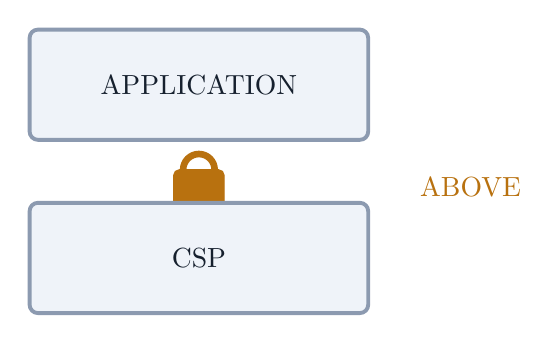
\begin{tikzpicture}
\draw[panel,line width=1.4pt] (0,3.2) rectangle (4.3,4.6); \node[lbli] at (2.15,3.9) {APPLICATION};
\lockicon{2.15}{2.6}{accent}
\node[lbl,text=accent] at (5.6,2.6) {ABOVE};
\draw[panel,line width=1.4pt] (0,1.0) rectangle (4.3,2.4); \node[lbli] at (2.15,1.7) {CSP};
\end{tikzpicture}}

\vspace{10pt}
\centering{\Large\color{ink}\bfseries CSP must remain, above.}
\vfill

\note{Here's the twist that makes this project interesting. Whatever we build, the application layer must keep talking plain CSP. Those applications are already flying, already qualified, and nobody is rewriting them for this.}
\end{frame}

% ============================== SLIDE 7 — TWIST, PART 2 ==============================
\begin{frame}{Two small issues}

\vfill
\bigfig[0.62\textheight]{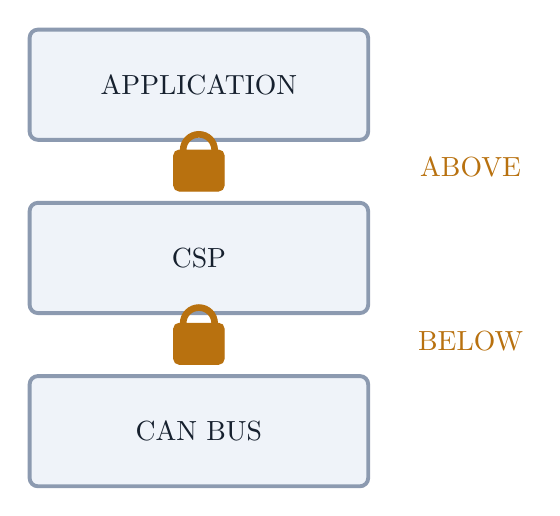
\begin{tikzpicture}
\draw[panel,line width=1.4pt] (0,4.9) rectangle (4.3,6.3); \node[lbli] at (2.15,5.6) {APPLICATION};
\lockicon{2.15}{4.55}{accent}
\node[lbl,text=accent] at (5.6,4.55) {ABOVE};
\draw[panel,line width=1.4pt] (0,2.7) rectangle (4.3,4.1); \node[lbli] at (2.15,3.4) {CSP};
\lockicon{2.15}{2.35}{accent}
\node[lbl,text=accent] at (5.6,2.35) {BELOW};
\draw[panel,line width=1.4pt] (0,0.5) rectangle (4.3,1.9); \node[lbli] at (2.15,1.2) {CAN BUS};
\end{tikzpicture}}

\vspace{10pt}
\centering{\Large\color{ink}\bfseries CSP must remain, above and below.}
\vfill

\note{And it's not just the application layer. The CAN bus underneath is the flight-proven, physical transport --- that can't be swapped out either. So CSP is pinned on both sides: above, at the application, and below, at the transport. Whatever carries DTN has to fit inside that sandwich.}
\end{frame}

% ============================== SLIDE 8 — CLIFFHANGER: NO PATH TODAY ==============================
\begin{frame}{The gap}

\vfill
\bigfig{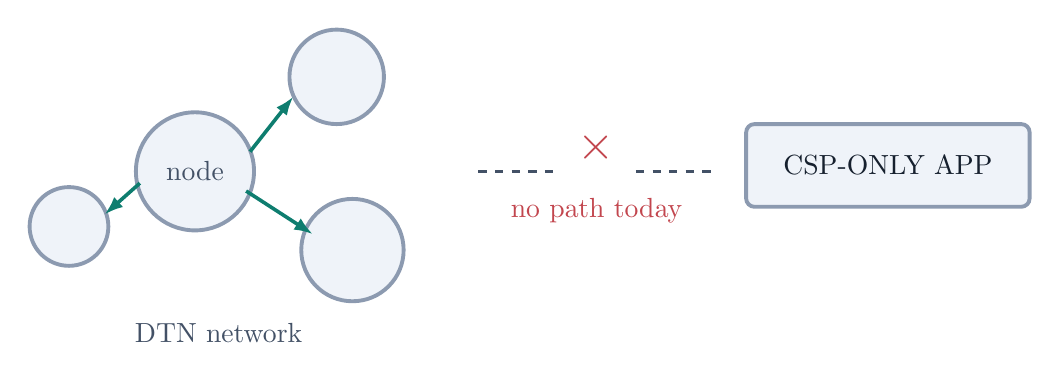
\begin{tikzpicture}
\draw[panel,line width=1.4pt] (0,1.3) circle (0.75); \node[lbl] at (0,1.3) {node};
\draw[panel,line width=1.4pt] (1.8,2.5) circle (0.6); \draw[panel,line width=1.4pt] (2.0,0.3) circle (0.65); \draw[panel,line width=1.4pt] (-1.6,0.6) circle (0.5);
\draw[accline] (0.7,1.55) -- (1.25,2.25);
\draw[accline] (0.65,1.05) -- (1.5,0.5);
\draw[accline] (-0.7,1.15) -- (-1.15,0.75);
\node[lbl] at (0.3,-0.75) {DTN network};

\draw[dimline] (3.6,1.3) -- (4.6,1.3);
\draw[dimline] (5.6,1.3) -- (6.6,1.3);
\node[font=\monofont\LARGE,text=warning] at (5.1,1.6) {$\times$};
\node[lbl,text=warning] at (5.1,0.8) {no path today};

\draw[panel,line width=1.4pt] (7,0.85) rectangle (10.6,1.9);
\node[lbli] at (8.8,1.375) {CSP-ONLY APP};
\end{tikzpicture}}
\vfill

\note{Here's the catch. If we bolt DTN on top of CSP, that's fine for brand-new applications written to talk BP. But every application already running directly on CSP has no idea BP exists, above or below. So the real research question is: how do you bring DTN to a CSP-based fleet, on both sides of that sandwich, without disrupting what's already flying?}
\end{frame}

% ============================== SLIDE 9 — WHY ABOVE ==============================
\begin{frame}{Why above}

\vfill
\begin{columns}[T]
\begin{column}{0.5\textwidth}\centering
\begin{cardbox}\centering\Large \led{accenttwo}\ \textbf{Zero rewrite}\end{cardbox}
\end{column}
\begin{column}{0.5\textwidth}\centering
\begin{cardbox}\centering\Large \led{accent}\ \textbf{Non-intrusive}\end{cardbox}
\end{column}
\end{columns}
\vfill

\note{Why must CSP remain above? Because legacy CSP-only applications are already flying, written and validated years ago, by a small team with no budget to rewrite and requalify them. Whatever we build has to be zero-rewrite, and non-intrusive to that code.}
\end{frame}

% ============================== SLIDE 10 — WHY BELOW ==============================
\begin{frame}{Why below}

\vfill
\begin{columns}[T]
\begin{column}{0.5\textwidth}\centering
\begin{cardbox}\centering\Large \led{accenttwo}\ \textbf{Real hardware}\end{cardbox}
\end{column}
\begin{column}{0.5\textwidth}\centering
\begin{cardbox}\centering\Large \led{accent}\ \textbf{Portable}\end{cardbox}
\end{column}
\end{columns}

\vspace{14pt}
\centering
\begin{cardbox}\centering\Large \led{accenttwo}\ Small teams. Small budgets.\end{cardbox}
\vfill

\note{Why must CSP remain below, on the CAN bus? Because the flight-proven avionics can't just be swapped out --- this has to run on the real RISC-V hardware CSUM flies, and be portable to whichever Bundle Protocol Agent ends up onboard. And underneath all of it: CSUM is a small team with a small budget, like most university-scale CubeSat operators. That's who this whole project is built for.}
\end{frame}

% ============================== SLIDE 11 — REVEAL: THE CSP-BP SANDWICH ==============================
\begin{frame}{The solution}

\vfill
\bigfig[0.4\textheight]{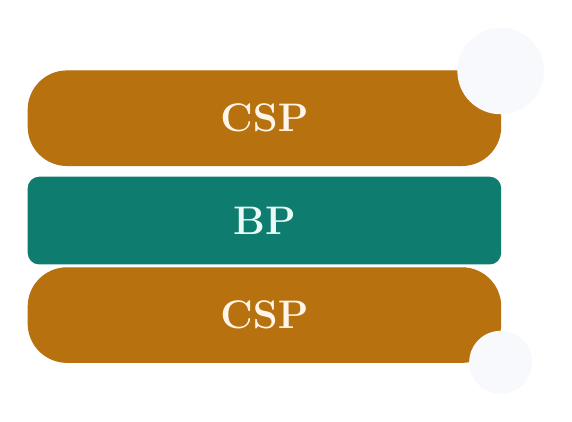
\begin{tikzpicture}
\draw[accent,fill=accent,rounded corners=14pt] (0,4.4) rectangle (6,5.6); \node[font=\monofont\Large\bfseries,text=accentinkon] at (3,5.0) {CSP};
\draw[accenttwo,fill=accenttwo,rounded corners=4pt] (0,3.15) rectangle (6,4.25); \node[font=\monofont\Large\bfseries,text=accenttwoinkon] at (3,3.7) {BP};
\draw[accent,fill=accent,rounded corners=14pt] (0,1.9) rectangle (6,3.1); \node[font=\monofont\Large\bfseries,text=accentinkon] at (3,2.5) {CSP};
\fill[bg] (6,5.6) circle (0.55);
\fill[bg] (6,1.9) circle (0.4);
\end{tikzpicture}}

\vspace{10pt}
\centering{\Large\color{ink}\bfseries The CSP-BP sandwich.}

\vspace{18pt}
\centering{\small\color{inkdim} Space agencies are already converging on BP}\\[8pt]
\chip{IOAG} \chip{NASA LCRNS} \chip{ESA Moonlight} \chip{NASA--ESA LunaNet}
\vfill

\note{Our answer: sandwich Bundle Protocol between two layers of CSP. CSP stays on top, talking to legacy applications unmodified. CSP stays on the bottom, riding the same CAN bus. And BP runs in the middle, getting bundles from one CSP layer to the other. We target Bundle Protocol specifically because it's where the space community is already converging: IOAG for Mars assets, NASA's LCRNS, ESA's Moonlight, and NASA-ESA LunaNet are all built around it.}
\end{frame}

% ============================== SLIDE 12 — CHARON: WHAT ==============================
\begin{frame}{Charon}

\vfill
\bigfig[0.42\textheight]{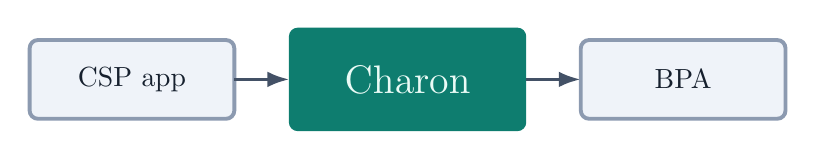
\begin{tikzpicture}
\draw[panel,line width=1.4pt] (0,1.2) rectangle (2.6,2.2); \node[lbli] at (1.3,1.7) {CSP app};
\draw[arrline] (2.6,1.7) -- (3.3,1.7);
\draw[accenttwobox] (3.3,1.05) rectangle (6.3,2.35); \node[font=\monofont\Large,text=accenttwoinkon] at (4.8,1.7) {Charon};
\draw[arrline] (6.3,1.7) -- (7.0,1.7);
\draw[panel,line width=1.4pt] (7.0,1.2) rectangle (9.6,2.2); \node[lbli] at (8.3,1.7) {BPA};
\end{tikzpicture}}

\vspace{16pt}
\centering{\Large\color{ink}\bfseries A tunnel: CSP, over Bundle Protocol.}
\vfill

\note{Charon is our answer for the application layer. It's a lightweight proxy that sits next to a CSP application and tunnels its traffic over Bundle Protocol, so the application itself never has to speak BP.}
\end{frame}

% ============================== SLIDE 13 — CHARON: WHY ==============================
\begin{frame}{Why Charon}

\vfill
\begin{columns}[c]
\begin{column}{0.46\textwidth}\centering
\bigfig[0.4\textheight]{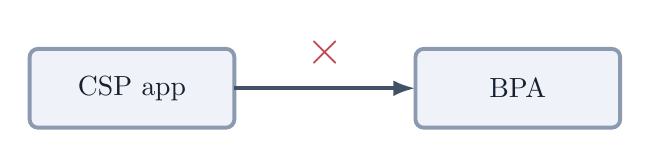
\begin{tikzpicture}
\draw[panel,line width=1.4pt] (0,1.2) rectangle (2.6,2.2); \node[lbli] at (1.3,1.7) {CSP app};
\draw[arrline] (2.6,1.7) -- (4.9,1.7);
\node[font=\monofont\LARGE,text=warning] at (3.75,2.15) {$\times$};
\draw[panel,line width=1.4pt] (4.9,1.2) rectangle (7.5,2.2); \node[lbli] at (6.2,1.7) {BPA};
\end{tikzpicture}}

\vspace{6pt}
{\small\color{warning} rewritten, or no DTN}
\end{column}
\begin{column}{0.46\textwidth}\centering
\bigfig[0.4\textheight]{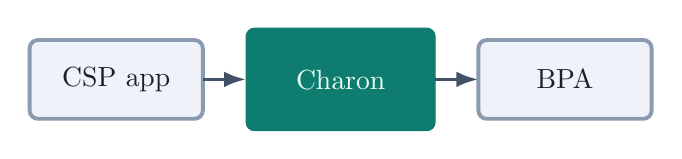
\begin{tikzpicture}
\draw[panel,line width=1.4pt] (0,1.2) rectangle (2.2,2.2); \node[lbli] at (1.1,1.7) {CSP app};
\draw[arrline] (2.2,1.7) -- (2.75,1.7);
\draw[accenttwobox] (2.75,1.05) rectangle (5.15,2.35); \node[font=\monofont\normalsize,text=accenttwoinkon] at (3.95,1.7) {Charon};
\draw[arrline] (5.15,1.7) -- (5.7,1.7);
\draw[panel,line width=1.4pt] (5.7,1.2) rectangle (7.9,2.2); \node[lbli] at (6.8,1.7) {BPA};
\end{tikzpicture}}

\vspace{6pt}
{\small\color{accenttwo} unchanged, and DTN}
\end{column}
\end{columns}
\vfill

\note{Why does Charon need to exist at all? Because without it, a legacy CSP application either gets rewritten to speak BP directly, which we ruled out, or it never benefits from DTN at all. Charon is what lets that application keep its code unchanged and still get store-and-forward delivery.}
\end{frame}

% ============================== SLIDE 14 — CHARON: HOW ==============================
\begin{frame}{How Charon works}

\vfill
\bigfig[0.6\textheight]{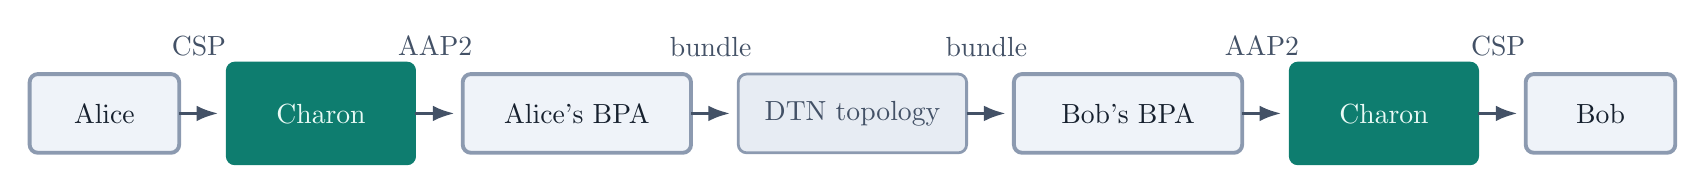
\begin{tikzpicture}[font=\monofont\normalsize]
\draw[panel,line width=1.4pt] (0,1.2) rectangle (1.9,2.2); \node[lbli] at (0.95,1.7) {Alice};
\draw[accenttwobox] (2.5,1.05) rectangle (4.9,2.35); \node[text=accenttwoinkon] at (3.7,1.7) {Charon};
\draw[panel,line width=1.4pt] (5.5,1.2) rectangle (8.4,2.2); \node[lbli] at (6.95,1.7) {Alice's BPA};
\draw[panel2] (9.0,1.2) rectangle (11.9,2.2); \node[text=inkdim] at (10.45,1.7) {DTN topology};
\draw[panel,line width=1.4pt] (12.5,1.2) rectangle (15.4,2.2); \node[lbli] at (13.95,1.7) {Bob's BPA};
\draw[accenttwobox] (16.0,1.05) rectangle (18.4,2.35); \node[text=accenttwoinkon] at (17.2,1.7) {Charon};
\draw[panel,line width=1.4pt] (19.0,1.2) rectangle (20.9,2.2); \node[lbli] at (19.95,1.7) {Bob};

\draw[arrline] (1.9,1.7) -- (2.4,1.7); \draw[arrline] (4.9,1.7) -- (5.4,1.7);
\draw[arrline] (8.4,1.7) -- (8.9,1.7); \draw[arrline] (11.9,1.7) -- (12.4,1.7);
\draw[arrline] (15.4,1.7) -- (15.9,1.7); \draw[arrline] (18.4,1.7) -- (18.9,1.7);

\node[text=inkdim] at (2.15,2.55) {CSP}; \node[text=inkdim] at (5.15,2.55) {AAP2};
\node[text=inkdim] at (8.65,2.55) {bundle}; \node[text=inkdim] at (12.15,2.55) {bundle};
\node[text=inkdim] at (15.65,2.55) {AAP2}; \node[text=inkdim] at (18.65,2.55) {CSP};
\end{tikzpicture}}

\vspace{16pt}
\centering\milestone{LEVEL 1 REACHED}
\vfill

\note{Charon is a lightweight tunnel that proxies IP, CAN, or CSP traffic over Bundle Protocol. In CSP mode, Alice's application talks plain CSP to her local Charon instance, which forwards it to her BPA over µD3TN's AAP2 interface. The bundle crosses the DTN topology, and on the other side Bob's BPA hands it to his Charon, which replays it to Bob as ordinary CSP. Neither application changed at all. That's our first milestone: CSP traffic itself now riding over a DTN network.}
\end{frame}

% ============================== SLIDE 15 — CSPCL: WHAT ==============================
\begin{frame}{CSPCL}

\vfill
\bigfig[0.6\textheight]{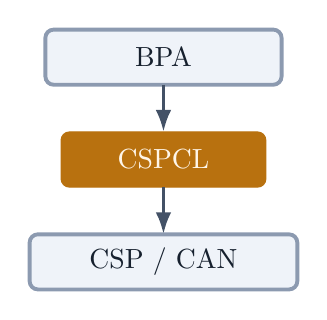
\begin{tikzpicture}
\draw[panel,line width=1.4pt] (0.7,4.65) rectangle (3.7,5.35); \node[lbli] at (2.2,5.0) {BPA};
\draw[arrline] (2.2,4.65) -- (2.2,4.05);
\draw[accentbox] (0.9,3.35) rectangle (3.5,4.05); \node[font=\monofont\normalsize,text=accentinkon] at (2.2,3.7) {CSPCL};
\draw[arrline] (2.2,3.35) -- (2.2,2.75);
\draw[panel,line width=1.4pt] (0.5,2.05) rectangle (3.9,2.75); \node[lbli] at (2.2,2.4) {CSP / CAN};
\end{tikzpicture}}

\vspace{16pt}
\centering{\Large\color{ink}\bfseries A Convergence Layer Adapter: bundles, over CSP.}
\vfill

\note{CSPCL is our answer for the transport layer. It's a Convergence Layer Adapter --- it lets a Bundle Protocol Agent speak CSP as its transport, so DTN nodes can talk to each other, or to CSP hardware, using the CAN bus that's already there.}
\end{frame}

% ============================== SLIDE 16 — CSPCL: WHY ==============================
\begin{frame}{Why CSPCL}

\vfill
\centering{\Huge\color{ink}\bfseries BP needs a ride.\\ CSP is the road.}
\vfill

\note{Why does CSPCL need to exist? Because on the transport side, there is no new hardware coming, and no new radio link. If Bundle Protocol is going to move at all on this fleet, it moves over the CSP and CAN that are already there. CSPCL is what makes that possible, and portable across whichever BPA ends up flying.}
\end{frame}

% ============================== SLIDE 17 — CSPCL: HOW (MECHANISM) ==============================
\begin{frame}{How CSPCL works}

\vfill
\bigfig[0.7\textheight]{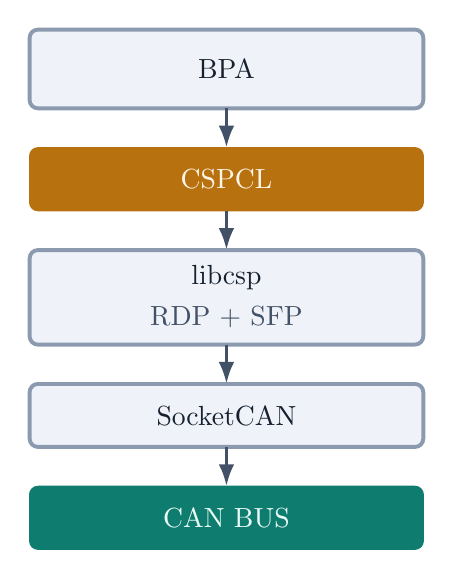
\begin{tikzpicture}
\draw[panel,line width=1.4pt] (0,7.7) rectangle (5,8.7); \node[lbli] at (2.5,8.2) {BPA};
\draw[arrline] (2.5,7.7) -- (2.5,7.2);
\draw[accentbox] (0,6.4) rectangle (5,7.2); \node[font=\monofont\normalsize,text=accentinkon] at (2.5,6.8) {CSPCL};
\draw[arrline] (2.5,6.4) -- (2.5,5.9);
\draw[panel,line width=1.4pt] (0,4.7) rectangle (5,5.9); \node[lbli] at (2.5,5.55) {libcsp};
\node[font=\monofont\normalsize,text=inkdim] at (2.5,5.05) {RDP + SFP};
\draw[arrline] (2.5,4.7) -- (2.5,4.2);
\draw[panel,line width=1.4pt] (0,3.4) rectangle (5,4.2); \node[lbli] at (2.5,3.8) {SocketCAN};
\draw[arrline] (2.5,3.4) -- (2.5,2.9);
\draw[accenttwobox] (0,2.1) rectangle (5,2.9); \node[font=\monofont\normalsize,text=accenttwoinkon] at (2.5,2.5) {CAN BUS};
\end{tikzpicture}}

\vspace{16pt}
\centering\milestone{LEVEL 2 REACHED}
\vfill

\note{Mechanically, a Convergence Layer Adapter's job is to map bundle transmission onto some underlying transport, the way TCPCL maps it onto TCP. CSPCL does that for CSP. It leans on two CSP features: RDP for acknowledged connections, and SFP for fragmentation, because a bundle is almost always bigger than a single CSP packet's MTU. And it integrates CAN as a physical transport via SocketCAN, so bundles ride the exact same wire the satellite already uses. That's our second milestone: libcspcl, a reusable engine any BPA can use to get a CSP convergence layer, cheaply.}
\end{frame}

% ============================== SLIDE 18 — CSPCL: HOW (RELIABILITY + PORTABILITY) ==============================
\begin{frame}{CSPCL --- reliability \& portability}

\vfill
\begin{columns}[c]
\begin{column}{0.52\textwidth}\centering
\bigfig[0.8\textheight]{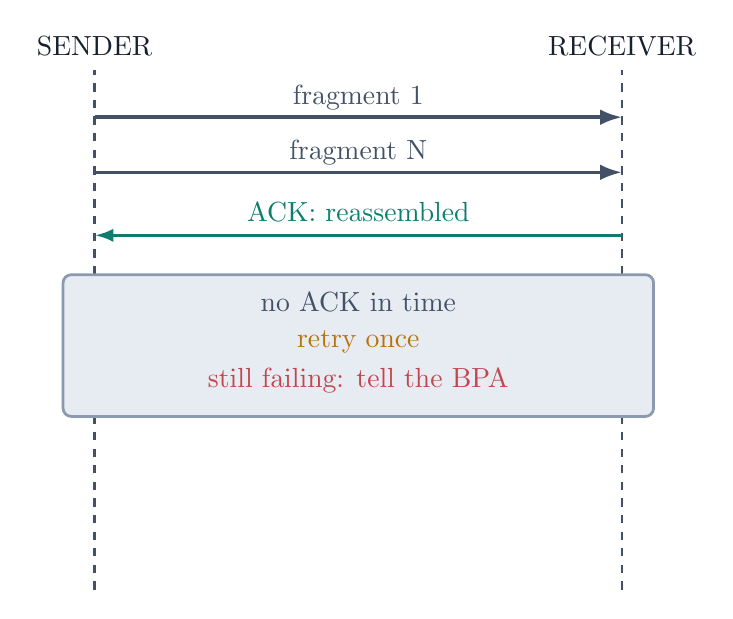
\begin{tikzpicture}
\node[lbli] at (0.8,7.1) {SENDER}; \node[lbli] at (7.5,7.1) {RECEIVER};
\draw[dimline] (0.8,0.2) -- (0.8,6.8);
\draw[dimline] (7.5,0.2) -- (7.5,6.8);
\draw[arrline] (0.8,6.2) -- (7.5,6.2); \node[lblf] at (4.15,6.45) {fragment 1};
\draw[arrline] (0.8,5.5) -- (7.5,5.5); \node[lblf] at (4.15,5.75) {fragment N};
\draw[accline] (7.5,4.7) -- (0.8,4.7);
\node[font=\monofont\normalsize,text=accenttwo] at (4.15,5.0) {ACK: reassembled};
\draw[panel2] (0.4,2.4) rectangle (7.9,4.2);
\node[lbl] at (4.15,3.85) {no ACK in time};
\node[font=\monofont\normalsize,text=accent] at (4.15,3.35) {retry once};
\node[font=\monofont\normalsize,text=warning] at (4.15,2.85) {still failing: tell the BPA};
\end{tikzpicture}}
\end{column}
\begin{column}{0.44\textwidth}\centering
\bigfig[0.6\textheight]{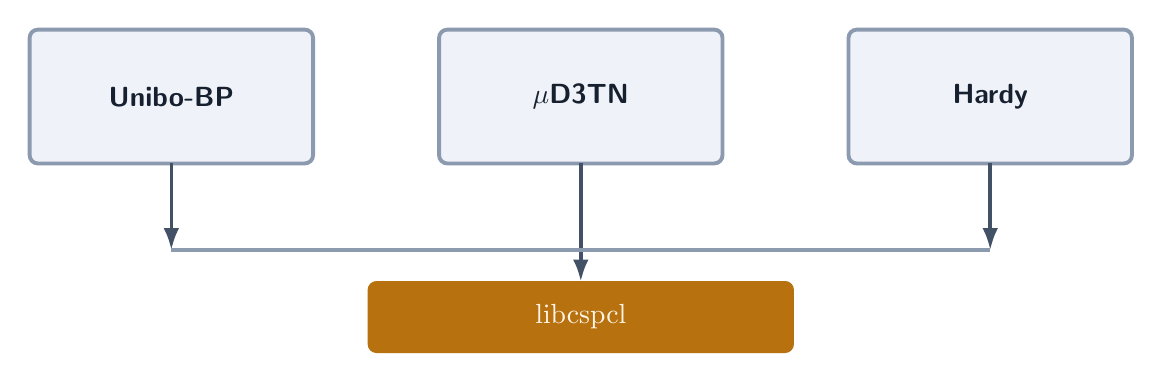
\begin{tikzpicture}
\draw[panel,line width=1.4pt] (0,3.6) rectangle (3.6,5.3); \node[font=\sffamily\bfseries,text=ink] at (1.8,4.45) {Unibo-BP};
\draw[panel,line width=1.4pt] (5.2,3.6) rectangle (8.8,5.3); \node[font=\sffamily\bfseries,text=ink] at (7.0,4.45) {\muD};
\draw[panel,line width=1.4pt] (10.4,3.6) rectangle (14.0,5.3); \node[font=\sffamily\bfseries,text=ink] at (12.2,4.45) {Hardy};
\draw[arrline] (1.8,3.6) -- (1.8,2.5);
\draw[arrline] (7.0,3.6) -- (7.0,2.1);
\draw[arrline] (12.2,3.6) -- (12.2,2.5);
\draw[line,line width=1.2pt] (1.8,2.5) -- (12.2,2.5);
\draw[accentbox] (4.3,1.2) rectangle (9.7,2.1);
\node[font=\monofont\normalsize,text=accentinkon] at (7.0,1.65) {libcspcl};
\end{tikzpicture}}

\vspace{10pt}
\milestone{LEVEL 3 REACHED}
\end{column}
\end{columns}
\vfill

\note{Two more things worth knowing. First, reliability: CSP's own acknowledgements only confirm a packet was handed off, not that the far end reassembled the whole bundle --- so CSPCL adds its own end-to-end ACK, retries once, and reports up to the BPA if it still fails. Second, portability: we integrated the same behavioral core into three structurally different BPAs --- Unibo-BP as a standalone daemon, µD3TN in-process, Hardy via an async Rust FFI binding. Same semantics, three very different integration shapes. That's our third milestone: BP and DTN traffic genuinely flowing over a CSP network, on three independent BPAs.}
\end{frame}

% ============================== SLIDE 19 — HARDWARE ==============================
\begin{frame}{The testbed}

\vfill
\bigfig[0.4\textheight]{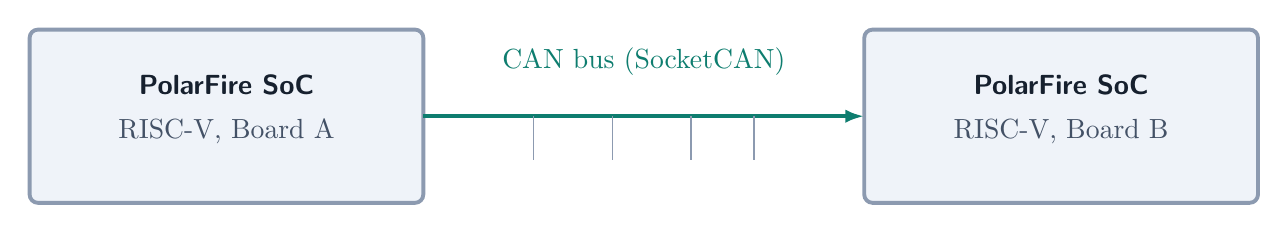
\begin{tikzpicture}
\draw[panel,line width=1.4pt] (0,0) rectangle (5,2.2); \node[font=\sffamily\bfseries,text=ink] at (2.5,1.5) {PolarFire SoC};
\node[lbl] at (2.5,0.9) {RISC-V, Board A};
\draw[panel,line width=1.4pt] (10.6,0) rectangle (15.6,2.2); \node[font=\sffamily\bfseries,text=ink] at (13.1,1.5) {PolarFire SoC};
\node[lbl] at (13.1,0.9) {RISC-V, Board B};
\draw[accline,line width=1.6pt] (5,1.1) -- (10.6,1.1);
\foreach \x in {6.4,7.4,8.4,9.2} \draw[line] (\x,1.1) -- (\x,0.55);
\node[font=\monofont\normalsize,text=accenttwo] at (7.8,1.8) {CAN bus (SocketCAN)};
\end{tikzpicture}}

\vspace{18pt}
\centering\photo{0.4\linewidth}{0.32\textheight}{polarfire_boards.png}
\vfill

\note{We didn't just validate this in simulation. Two Microchip PolarFire SoC RISC-V development boards, wired together over a real CAN bus, running SocketCAN --- exactly the real-hardware requirement from earlier, and it mirrors the actual avionics architecture of CSUM's upcoming 12U CubeSat mission. On this hardware we validated two Hardy nodes talking through CSPCL with A-SABR routing, and two Unibo-BP nodes doing the same.}
\end{frame}

% ============================== SLIDE 20 — DEMO: FOUR-NODE CHAIN ==============================
\begin{frame}{The full chain}

\vfill
\bigfig{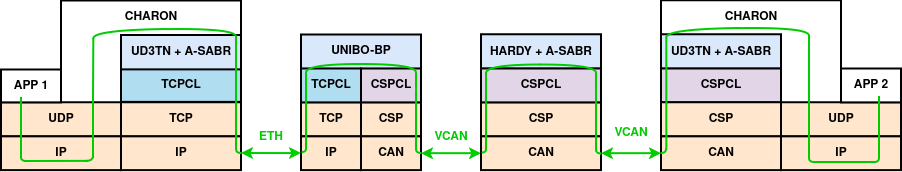
\includegraphics{full_chain.png}}
\vfill

\note{For the full end-to-end test we built a four-node chain where every single hop uses a different transport-and-BPA combination on purpose --- maximum heterogeneity. Alice is µD3TN with an A-SABR routing engine, bridging IP traffic in through Charon and out over TCPCL. Unibo-BP receives that over TCPCL and forwards it onto a virtual CAN bus via CSPCL. Hardy talks CAN on both sides. And it lands on Bob, µD3TN again, which hands it back to Charon and out to the receiving application.}
\end{frame}

% ============================== SLIDE 21 — STATS: FRAMING OVERHEAD ==============================
\begin{frame}{Framing overhead}

\vfill
\bigfig[0.66\textheight]{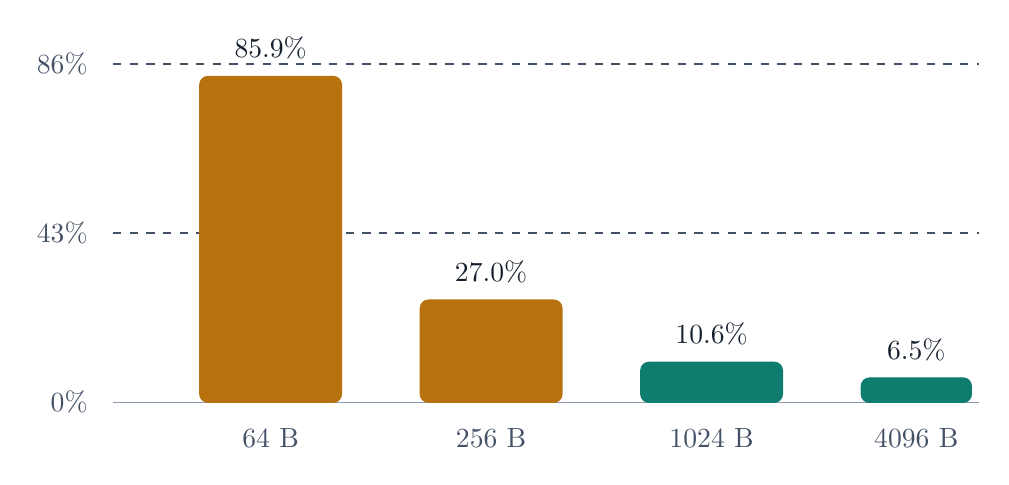
\begin{tikzpicture}
\draw[line] (0,0) -- (11,0);
\draw[dimline] (0,4.3) -- (11,4.3); \node[lblf,anchor=east] at (-0.2,4.3) {86\%};
\draw[dimline] (0,2.15) -- (11,2.15); \node[lblf,anchor=east] at (-0.2,2.15) {43\%};
\node[lblf,anchor=east] at (-0.2,0) {0\%};

\draw[accentbox] (1.1,0) rectangle (2.9,4.14);
\node[lbli] at (2.0,4.5) {85.9\%};
\node[lbl] at (2.0,-0.45) {64 B};

\draw[accentbox] (3.9,0) rectangle (5.7,1.30);
\node[lbli] at (4.8,1.66) {27.0\%};
\node[lbl] at (4.8,-0.45) {256 B};

\draw[accenttwobox] (6.7,0) rectangle (8.5,0.51);
\node[lbli] at (7.6,0.87) {10.6\%};
\node[lbl] at (7.6,-0.45) {1024 B};

\draw[accenttwobox] (9.5,0) rectangle (10.9,0.31);
\node[lbli] at (10.2,0.67) {6.5\%};
\node[lbl] at (10.2,-0.45) {4096 B};
\end{tikzpicture}}

\vspace{14pt}
\centering{\Large\color{ink}\bfseries Batch telemetry into bigger bundles.}
\vfill

\note{First the framing cost. A BP7 bundle carries CBOR framing overhead, and CSPCL fragments it further via SFP. At a tiny 64-byte payload that overhead is almost eighty-six percent of the bytes on the wire. But it falls fast: by 4096 bytes it's down to six and a half percent. The lesson for an operator: batch your telemetry into fewer, larger bundles whenever the mission allows it.}
\end{frame}

% ============================== SLIDE 22 — STATS: MTU SURPRISE ==============================
\begin{frame}{An MTU surprise}

\vfill
\begin{columns}[c]
\begin{column}{0.46\textwidth}
\centering
\bigfig[0.62\textheight]{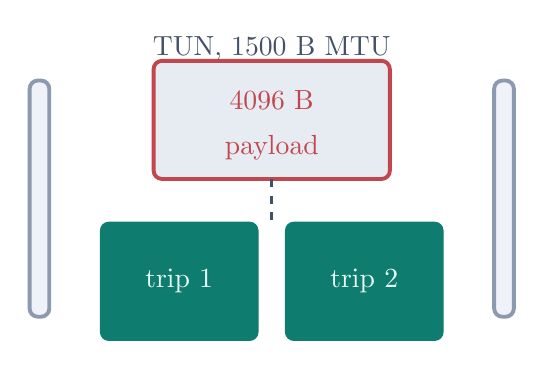
\begin{tikzpicture}
\draw[panel,line width=1.4pt] (0,2.4) rectangle (0.25,5.4);
\draw[panel,line width=1.4pt] (5.9,2.4) rectangle (6.15,5.4);
\node[lbl] at (3.075,5.8) {TUN, 1500 B MTU};
\draw[warnbox,line width=1.4pt] (1.575,4.15) rectangle (4.575,5.65);
\node[font=\monofont\normalsize,text=warning] at (3.075,5.15) {4096 B};
\node[font=\monofont\normalsize,text=warning] at (3.075,4.55) {payload};
\draw[dimline] (3.075,4.15) -- (3.075,3.6);
\draw[accenttwobox] (0.9,2.1) rectangle (2.9,3.6); \node[font=\monofont\normalsize,text=accenttwoinkon] at (1.9,2.85) {trip 1};
\draw[accenttwobox] (3.25,2.1) rectangle (5.25,3.6); \node[font=\monofont\normalsize,text=accenttwoinkon] at (4.25,2.85) {trip 2};
\end{tikzpicture}}
\end{column}
\begin{column}{0.5\textwidth}
\centering
\bigfig[0.62\textheight]{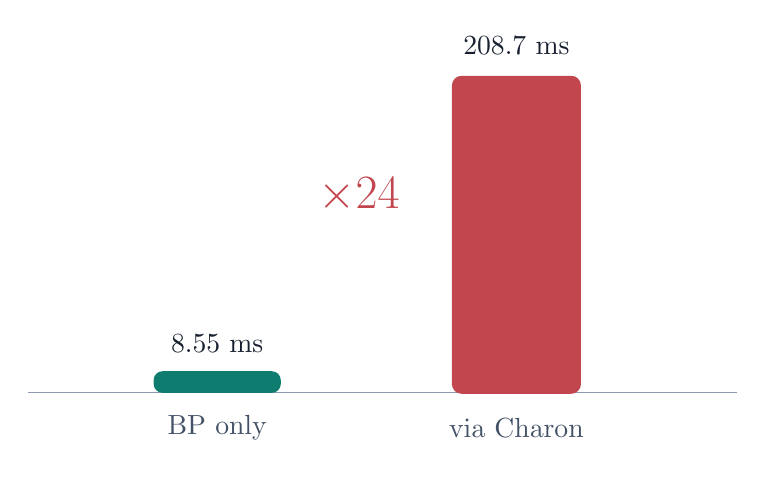
\begin{tikzpicture}
\draw[line] (0,0) -- (9,0);
\draw[accenttwobox] (1.6,0) rectangle (3.2,0.26); \node[lbli] at (2.4,0.62) {8.55 ms};
\node[lbl] at (2.4,-0.45) {BP only};
\draw[warnbox,fill=warning] (5.4,0) rectangle (7.0,4.0); \node[lbli] at (6.2,4.4) {208.7 ms};
\node[lbl] at (6.2,-0.45) {via Charon};
\node[font=\monofont\LARGE,text=warning] at (4.2,2.5) {$\times$24};
\end{tikzpicture}}
\end{column}
\end{columns}
\vfill

\note{Here's a finding we didn't expect. Charon tracks the plain Bundle-Protocol latency closely up to 1024 bytes. But at 4096 bytes, its latency jumps roughly twenty-four times. We dug in: Charon's IP mode reads from a Linux TUN interface with the default 1500-byte MTU. A 4096-byte payload doesn't fit through that door in one trip, so the kernel silently fragments it into multiple IP packets, each independently tunneled over the same bundle hop. A real, measured cost of the IP-tunneling design.}
\end{frame}

% ============================== SLIDE 23 — STATS: THROUGHPUT & DELIVERY ==============================
\begin{frame}{Throughput \& delivery}

\vfill
\bigfig[0.5\textheight]{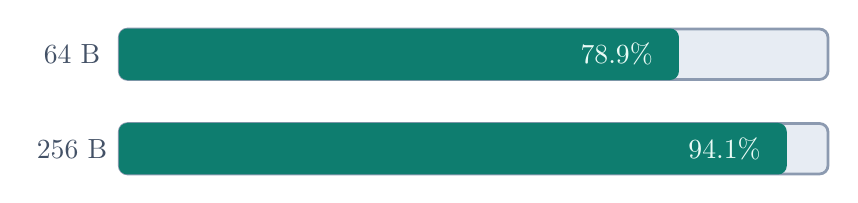
\begin{tikzpicture}
\node[lbl] at (-0.6,1.6) {64 B};
\draw[panel2] (0,1.28) rectangle (9,1.92);
\draw[accenttwobox] (0,1.28) rectangle (7.10,1.92);
\node[font=\monofont\normalsize,text=accenttwoinkon,anchor=east] at (6.9,1.6) {78.9\%};

\node[lbl] at (-0.6,0.4) {256 B};
\draw[panel2] (0,0.08) rectangle (9,0.72);
\draw[accenttwobox] (0,0.08) rectangle (8.47,0.72);
\node[font=\monofont\normalsize,text=accenttwoinkon,anchor=east] at (8.27,0.4) {94.1\%};
\end{tikzpicture}}

\vspace{10pt}
\centering{\small\color{inkdim} 78.9\% and 94.1\% are throughput as \% of the contact plan's modeled ceiling}

\vspace{18pt}
\centering\chipstrong{100\% delivery}\\[6pt]
\centering{\small\color{inkdim} over 100 iterations}
\vfill

\note{Zooming back out to the full four-node chain, shaped down to the contact plan's modeled rates: delivery was completely reliable at both payload sizes we tested. Achieved throughput reached seventy-nine to ninety-four percent of the theoretical ceiling, which lines up with the per-hop overhead we just saw, compounded across three hops and two independent routing decisions.}
\end{frame}

% ============================== SLIDE 24 — STATS: DISRUPTION TEST ==============================
\begin{frame}{Disruption test}

\vfill
\centering
\begin{tcolorbox}[colback=bgpanel2, colframe=line, boxrule=0.8pt, arc=6pt,
  left=18pt,right=18pt,top=16pt,bottom=16pt, width=0.85\linewidth]
{\monofont\Large
\textcolor{inkdim}{\$} \textcolor{ink}{kill -9 unibo-bp-cspcl}\\[10pt]
\textcolor{accent}{[bundle]} \textcolor{ink}{held in storage}\\[10pt]
\textcolor{accenttwo}{[unibo-bp-cspcl]} \textcolor{ink}{restarted}\\[10pt]
\textcolor{accenttwo}{[bundle]} \textcolor{ink}{delivered}
}
\end{tcolorbox}

\vspace{22pt}
{\Large\color{accenttwo}\bfseries Store-and-forward, validated.}
\vfill

\note{And then we tried to break it on purpose. We killed the unibo-bp-cspcl daemon outright, mid-transfer, discarding its entire connection-pool state, and left it dead for a few seconds while bundles were in flight. Traffic aimed at the disrupted node was simply held in storage by its neighbor. The moment the daemon came back, delivery resumed and completed, no data lost.}
\end{frame}

% ============================== SLIDE 25 — LIMITATIONS \& FUTURE: ABOVE (CHARON) ==============================
\begin{frame}{Charon --- above}

\vfill
\begin{cardbox}
\Large
\led{accent}\ \textbf{\color{ink}Single BPA support}
\vspace{10pt}\hrule height 0.4pt \color{linesoft}\vspace{10pt}
\led{accent}\ \textbf{\color{ink}No local packet queue}
\vspace{10pt}\hrule height 0.4pt \color{linesoft}\vspace{10pt}
\led{accent}\ \textbf{\color{ink}No CSP routing in CSP mode}
\vspace{10pt}\hrule height 0.4pt \color{linesoft}\vspace{10pt}
\led{accenttwo}\ \textbf{\color{ink}Next: beyond \muD}
\end{cardbox}
\vfill

\note{On the Charon side: it only integrates directly with µD3TN today, through AAP2. It has no packet buffer of its own, so if the BPA is briefly unavailable, in-flight packets are dropped, not queued. And CSP mode gives point-to-point association between two named peers, not general CSP routing across the DTN topology. Next up: growing Charon's BPA support beyond µD3TN, to Unibo-BP, Hardy, and ION-DTN.}
\end{frame}

% ============================== SLIDE 26 — LIMITATIONS \& FUTURE: BELOW (CSPCL) ==============================
\begin{frame}{CSPCL --- below}

\vfill
\begin{cardbox}
\Large
\led{accenttwo}\ \textbf{\color{ink}Use A-SABR for routing}
\vspace{10pt}\hrule height 0.4pt \color{linesoft}\vspace{10pt}
\led{accenttwo}\ \textbf{\color{ink}Next: micro-controller support}
\vspace{10pt}\hrule height 0.4pt \color{linesoft}\vspace{10pt}
\led{accenttwo}\ \textbf{\color{ink}Next: narrow the pool mutex}
\end{cardbox}
\vfill

\note{On the CSPCL side: the next step is to use A-SABR as the routing algorithm, so routing decisions stay aligned with the contact-plan logic used elsewhere in the stack. Next up: A-SABR is being ported to microcontrollers, and CSPCL should follow, so we can validate on CSUM's non-Linux CubeSats too. And on the engineering side, the connection pool's single mutex is the latency bottleneck we saw earlier --- narrowing its scope to just pool bookkeeping is the next fix.}
\end{frame}

% ============================== SLIDE 27 — THANK YOU ==============================
\begin{frame}[plain]
\vspace{18pt}
\eyebrow{Thank you}\\[16pt]
{\fontsize{44}{44}\selectfont\bfseries\color{ink} Questions?}\\[16pt]
{\Large\color{inkdim} Non-disruptive DTN adoption for CSP-based CubeSats.}\\[8pt]
{\large\color{accenttwo}\bfseries Not just a paper idea.}\\[20pt]

\chip{Mathias Durat} \chip{Sarah Theoulle} \chip{Hugo Ponthieu} \chip{Tristan-Mihai Radulescu} \chip{Olivier De Jonck\`ere}

\vspace{8pt}
\chip{LIRMM $\cdot$ Polytech Montpellier $\cdot$ CSUM}

\note{Thank you --- happy to take questions, whether about the CLA internals, the Charon proxy, or the evaluation setup.}
\end{frame}

\end{document}
